\begin{figure}[p]
\centering
\captionsetup{justification=raggedright,labelsep=none,singlelinecheck=false,labelformat=boldlabel}
\caption[]{\footnotesize \textbf{: Decomposition of the equal-weighted forecast strategy's Sharpe ratio across the 153 factors.} The bars show the cross-sectional mean raw Sharpe ratio, the change associated with capping exposure at 1.5, the change associated with transaction costs, and the resulting net capped Sharpe ratio. Error bars report the interquartile range across factors for the raw and final levels and for each intermediate change.}
\label{fig:rv-portfolio_ew_sharpe_waterfall}
\par\smallskip\textbf{Panel A. Long sample}\par\smallskip
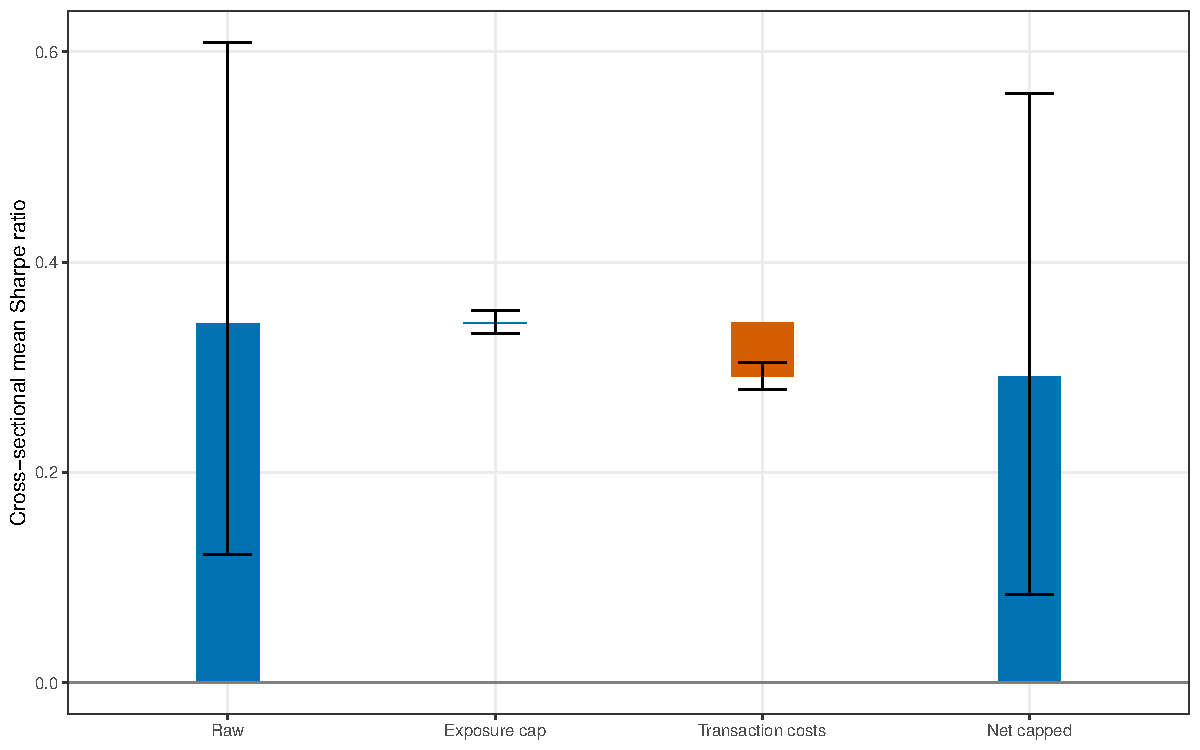
\includegraphics[width=\linewidth,height=0.70\textheight,keepaspectratio]{results_v3/1927/internet_appendix/portfolio_ew_sharpe_waterfall.pdf}
\end{figure}
\begin{figure}[p]
\ContinuedFloat
\centering
\captionsetup{justification=raggedright,labelsep=none,singlelinecheck=false,labelformat=boldlabel}
\caption[]{\footnotesize \textbf{: Decomposition of the equal-weighted forecast strategy's Sharpe ratio across the 153 factors.} The bars show the cross-sectional mean raw Sharpe ratio, the change associated with capping exposure at 1.5, the change associated with transaction costs, and the resulting net capped Sharpe ratio. Error bars report the interquartile range across factors for the raw and final levels and for each intermediate change. Continued.}
\par\smallskip\textbf{Panel B. Short sample}\par\smallskip
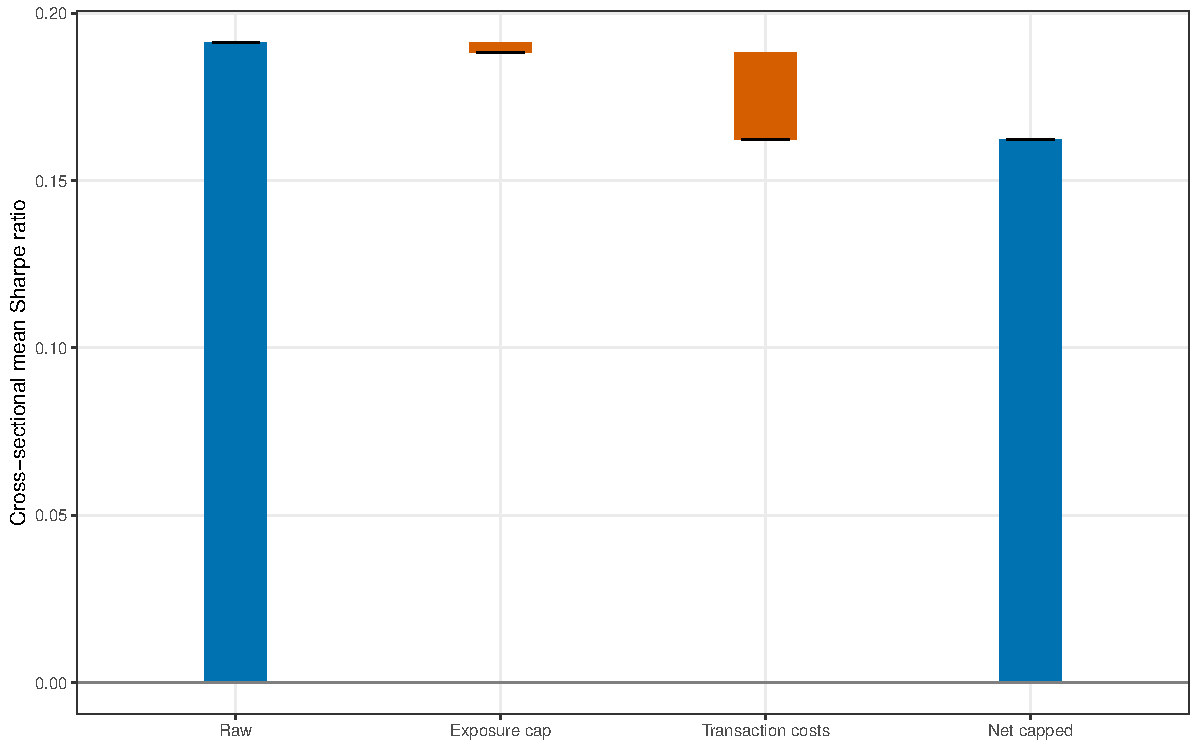
\includegraphics[width=\linewidth,height=0.70\textheight,keepaspectratio]{results_v3/1986/internet_appendix/portfolio_ew_sharpe_waterfall.pdf}
\end{figure}
